% !TeX program = xelatex 
%  LaTeX support: latex@mdpi.com 
%  For support, please attach all files needed for compiling as well as the log file, and specify your operating system, LaTeX version, and LaTeX editor.

%=================================================================
\documentclass[mathematics,article,submit,moreauthors]{Definitions/mdpi} 

%--------------------
% Class Options:
%--------------------
%----------
% journal
%----------
% Choose between the following MDPI journals:
% acoustics, actuators, addictions, admsci, adolescents, aerobiology, aerospace, agriculture, agriengineering, agrochemicals, agronomy, ai, air, algorithms, allergies, alloys, analytica, analytics, anatomia, animals, antibiotics, antibodies, antioxidants, applbiosci, appliedchem, appliedmath, applmech, applmicrobiol, applnano, applsci, aquacj, architecture, arm, arthropoda, arts, asc, asi, astronomy, atmosphere, atoms, audiolres, automation, axioms, bacteria, batteries, bdcc, behavsci, beverages, biochem, bioengineering, biologics, biology, biomass, biomechanics, biomed, biomedicines, biomedinformatics, biomimetics, biomolecules, biophysica, biosensors, biotech, birds, bloods, blsf, brainsci, breath, buildings, businesses, cancers, carbon, cardiogenetics, catalysts, cells, ceramics, challenges, chemengineering, chemistry, chemosensors, chemproc, children, chips, cimb, civileng, cleantechnol, climate, clinpract, clockssleep, cmd, coasts, coatings, colloids, colorants, commodities, compounds, computation, computers, condensedmatter, conservation, constrmater, cosmetics, covid, crops, cryptography, crystals, csmf, ctn, curroncol, cyber, dairy, data, ddc, dentistry, dermato, dermatopathology, designs, devices, diabetology, diagnostics, dietetics, digital, disabilities, diseases, diversity, dna, drones, dynamics, earth, ebj, ecologies, econometrics, economies, education, ejihpe, electricity, electrochem, electronicmat, electronics, encyclopedia, endocrines, energies, eng, engproc, entomology, entropy, environments, environsciproc, epidemiologia, epigenomes, est, fermentation, fibers, fintech, fire, fishes, fluids, foods, forecasting, forensicsci, forests, foundations, fractalfract, fuels, future, futureinternet, futurepharmacol, futurephys, futuretransp, galaxies, games, gases, gastroent, gastrointestdisord, gels, genealogy, genes, geographies, geohazards, geomatics, geosciences, geotechnics, geriatrics, grasses, gucdd, hazardousmatters, healthcare, hearts, hemato, hematolrep, heritage, higheredu, highthroughput, histories, horticulturae, hospitals, humanities, humans, hydrobiology, hydrogen, hydrology, hygiene, idr, ijerph, ijfs, ijgi, ijms, ijns, ijpb, ijtm, ijtpp, ime, immuno, informatics, information, infrastructures, inorganics, insects, instruments, inventions, iot, j, jal, jcdd, jcm, jcp, jcs, jcto, jdb, jeta, jfb, jfmk, jimaging, jintelligence, jlpea, jmmp, jmp, jmse, jne, jnt, jof, joitmc, jor, journalmedia, jox, jpm, jrfm, jsan, jtaer, jvd, jzbg, kidneydial, kinasesphosphatases, knowledge, land, languages, laws, life, liquids, literature, livers, logics, logistics, lubricants, lymphatics, machines, macromol, magnetism, magnetochemistry, make, marinedrugs, materials, materproc, mathematics, mca, measurements, medicina, medicines, medsci, membranes, merits, metabolites, metals, meteorology, methane, metrology, micro, microarrays, microbiolres, micromachines, microorganisms, microplastics, minerals, mining, modelling, molbank, molecules, mps, msf, mti, muscles, nanoenergyadv, nanomanufacturing,\gdef\@continuouspages{yes}} nanomaterials, ncrna, ndt, network, neuroglia, neurolint, neurosci, nitrogen, notspecified, %%nri, nursrep, nutraceuticals, nutrients, obesities, oceans, ohbm, onco, %oncopathology, optics, oral, organics, organoids, osteology, oxygen, parasites, parasitologia, particles, pathogens, pathophysiology, pediatrrep, pharmaceuticals, pharmaceutics, pharmacoepidemiology,\gdef\@ISSN{2813-0618}\gdef\@continuous pharmacy, philosophies, photochem, photonics, phycology, physchem, physics, physiologia, plants, plasma, platforms, pollutants, polymers, polysaccharides, poultry, powders, preprints, proceedings, processes, prosthesis, proteomes, psf, psych, psychiatryint, psychoactives, publications, quantumrep, quaternary, qubs, radiation, reactions, receptors, recycling, regeneration, religions, remotesensing, reports, reprodmed, resources, rheumato, risks, robotics, ruminants, safety, sci, scipharm, sclerosis, seeds, sensors, separations, sexes, signals, sinusitis, skins, smartcities, sna, societies, socsci, software, soilsystems, solar, solids, spectroscj, sports, standards, stats, std, stresses, surfaces, surgeries, suschem, sustainability, symmetry, synbio, systems, targets, taxonomy, technologies, telecom, test, textiles, thalassrep, thermo, tomography, tourismhosp, toxics, toxins, transplantology, transportation, traumacare, traumas, tropicalmed, universe, urbansci, uro, vaccines, vehicles, venereology, vetsci, vibration, virtualworlds, viruses, vision, waste, water, wem, wevj, wind, women, world, youth, zoonoticdis 
% For posting an early version of this manuscript as a preprint, you may use "preprints" as the journal. Changing "submit" to "accept" before posting will remove line numbers.

%---------
% article
%---------
% The default type of manuscript is "article", but can be replaced by: 
% abstract, addendum, article, book, bookreview, briefreport, casereport, comment, commentary, communication, conferenceproceedings, correction, conferencereport, entry, expressionofconcern, extendedabstract, datadescriptor, editorial, essay, erratum, hypothesis, interestingimage, obituary, opinion, projectreport, reply, retraction, review, perspective, protocol, shortnote, studyprotocol, systematicreview, supfile, technicalnote, viewpoint, guidelines, registeredreport, tutorial
% supfile = supplementary materials

%----------
% submit
%----------
% The class option "submit" will be changed to "accept" by the Editorial Office when the paper is accepted. This will only make changes to the frontpage (e.g., the logo of the journal will get visible), the headings, and the copyright information. Also, line numbering will be removed. Journal info and pagination for accepted papers will also be assigned by the Editorial Office.

%------------------
% moreauthors
%------------------
% If there is only one author the class option oneauthor should be used. Otherwise use the class option moreauthors.

%---------
% pdftex
%---------
% The option pdftex is for use with pdfLaTeX. Remove "pdftex" for (1) compiling with LaTeX & dvi2pdf (if eps figures are used) or for (2) compiling with XeLaTeX.

%=================================================================
% MDPI internal commands - do not modify
\firstpage{1} 
\makeatletter 
\setcounter{page}{\@firstpage} 
\makeatother
\pubvolume{1}
\issuenum{1}
\articlenumber{0}
\pubyear{2023}
\copyrightyear{2023}
%\externaleditor{Academic Editor: Firstname Lastname}
\datereceived{ } 
\daterevised{ } % Comment out if no revised date
\dateaccepted{ } 
\datepublished{ } 
%\datecorrected{} % For corrected papers: "Corrected: XXX" date in the original paper.
%\dateretracted{} % For corrected papers: "Retracted: XXX" date in the original paper.
\hreflink{https://doi.org/} % If needed use \linebreak
%\doinum{}
%\pdfoutput=1 % Uncommented for upload to arXiv.org

%=================================================================
% Add packages and commands here. The following packages are loaded in our class file: fontenc, inputenc, calc, indentfirst, fancyhdr, graphicx, epstopdf, lastpage, ifthen, float, amsmath, amssymb, lineno, setspace, enumitem, mathpazo, booktabs, titlesec, etoolbox, tabto, xcolor, colortbl, soul, multirow, microtype, tikz, totcount, changepage, attrib, upgreek, array, tabularx, pbox, ragged2e, tocloft, marginnote, marginfix, enotez, amsthm, natbib, hyperref, cleveref, scrextend, url, geometry, newfloat, caption, draftwatermark, seqsplit
% cleveref: load \crefname definitions after \begin{document}

%=================================================================
% Please use the following mathematics environments: Theorem, Lemma, Corollary, Proposition, Characterization, Property, Problem, Example, ExamplesandDefinitions, Hypothesis, Remark, Definition, Notation, Assumption
%% For proofs, please use the proof environment (the amsthm package is loaded by the MDPI class).

%=================================================================
% Full title of the paper (Capitalized)
%\Title{Expansive Information Injection with Large Language Models for Multi-Span Question Answering }
\Title{Empowering Multi-Span Question Answering with Expansive Information Injection using Large Language Models}

% MDPI internal command: Title for citation in the left column
\TitleCitation{Title}

% Author Orchid ID: enter ID or remove command
\newcommand{\orcidauthorA}{0000-0002-2206-1926} % Add \orcidA{} behind the author's name
%\newcommand{\orcidauthorB}{0000-0000-0000-000X} % Add \orcidB{} behind the author's name


% Authors, for the paper (add full first names)
\Author{Zhiyi Luo $^{1}$\orcidA{}, Yingying Zhang$^{1}$ and Shuyun Luo $^{1,}$*}

%\longauthorlist{yes}

% MDPI internal command: Authors, for metadata in PDF
\AuthorNames{Zhiyi Luo, Yingying Zhang and Shuyun Luo}

% MDPI internal command: Authors, for citation in the left column
\AuthorCitation{Luo, Z.; Zhang, Y.; Luo, S.}
% If this is a Chicago style journal: Lastname, Firstname, Firstname Lastname, and Firstname Lastname.

% Affiliations / Addresses (Add [1] after \address if there is only one affiliation.)
\address{%
$^{1}$ \quad School of Computer Science and Technology and the Key Laboratory of Intelligent Textile and Flexible Interconnection of Zhejiang Province, Zhejiang Sci-Tech University, Hangzhou, China; luozhiyi@zstu.edu.cn
%$^{2}$ \quad Affiliation 2; e-mail@e-mail.com
}

% Contact information of the corresponding author
\corres{Correspondence: shuyunluo@zstu.edu.cn;}

% Current address and/or shared authorship
%\firstnote{Current address: Affiliation 3.} 
%\secondnote{These authors contributed equally to this work.}
% The commands \thirdnote{} till \eighthnote{} are available for further notes

%\simplesumm{} % Simple summary

%\conference{} % An extended version of a conference paper

% Abstract (Do not insert blank lines, i.e. \\) 
\abstract{Retrieval-based question answering in the automotive domain requires a model to comprehend and articulate relevant domain knowledge, accurately understand user intent, and effectively match the required information. Typically, these systems employ a encoder-retriever architecture. However, existing encoders, which rely on pretrained language models, suffer from limited specialization, insufficient awareness of domain knowledge, and biases in user intent understanding. To overcome these limitations, this paper constructs a Chinese corpus specifically tailored for the automotive domain, comprising question-answer pairs, document collections, and multitask annotated data. Subsequently, a pretraining-multitask fine-tuning framework based on masked language models is introduced to integrate domain knowledge as well as enhance semantic representations, thereby yielding benefits for downstream applications. To evaluate system performance, an evaluation dataset is created using ChatGPT, and a novel retrieval task evaluation metric called Mean Linear Window Rank (MLWR) is proposed. Experimental results demonstrate that the proposed system (based on $\text{BERT}_{base}$), achieves accuracies of 77.5\% and 84.75\% for Hit@1 and Hit@3 respectively, in the automotive domain retrieval-based question answering task. Additionally, the MLWR reaches 87.71\%. Compared to a system utilizing a general encoder, the proposed multitask fine-tuning strategy shows improvements of 12.5\%, 12.5\%, and 28.16\% for Hit@1, Hit@3, and MLWR, respectively. Furthermore, when compared to the best single-task fine-tuning strategy, the enhancements amount to 0.5\%, 1.25\%, and 0.95\% for Hit@1, Hit@3, and MLWR, respectively.}

% Keywords
\keyword{deep learning; pretrained language model; retrieval-based question answering; multitask learning; fine-tuning} 

% The fields PACS, MSC, and JEL may be left empty or commented out if not applicable
%\PACS{J0101}
%\MSC{}
%\JEL{}

%%%%%%%%%%%%%%%%%%%%%%%%%%%%%%%%%%%%%%%%%%
% Only for the journal Diversity
%\LSID{\url{http://}}

%%%%%%%%%%%%%%%%%%%%%%%%%%%%%%%%%%%%%%%%%%
% Only for the journal Applied Sciences
%\featuredapplication{Authors are encouraged to provide a concise description of the specific application or a potential application of the work. This section is not mandatory.}
%%%%%%%%%%%%%%%%%%%%%%%%%%%%%%%%%%%%%%%%%%

%%%%%%%%%%%%%%%%%%%%%%%%%%%%%%%%%%%%%%%%%%
% Only for the journal Data
%\dataset{DOI number or link to the deposited data set if the data set is published separately. If the data set shall be published as a supplement to this paper, this field will be filled by the journal editors. In this case, please submit the data set as a supplement.}
%\datasetlicense{License under which the data set is made available (CC0, CC-BY, CC-BY-SA, CC-BY-NC, etc.)}

%%%%%%%%%%%%%%%%%%%%%%%%%%%%%%%%%%%%%%%%%%
% Only for the journal Toxins
%\keycontribution{The breakthroughs or highlights of the manuscript. Authors can write one or two sentences to describe the most important part of the paper.}

%%%%%%%%%%%%%%%%%%%%%%%%%%%%%%%%%%%%%%%%%%
% Only for the journal Encyclopedia
%\encyclopediadef{For entry manuscripts only: please provide a brief overview of the entry title instead of an abstract.}

%%%%%%%%%%%%%%%%%%%%%%%%%%%%%%%%%%%%%%%%%%
% Only for the journal Advances in Respiratory Medicine
%\addhighlights{yes}
%\renewcommand{\addhighlights}{%

%\noindent This is an obligatory section in “Advances in Respiratory Medicine”, whose goal is to increase the discoverability and readability of the article via search engines and other scholars. Highlights should not be a copy of the abstract, but a simple text allowing the reader to quickly and simplified find out what the article is about and what can be cited from it. Each of these parts should be devoted up to 2~bullet points.\vspace{3pt}\\
%\textbf{What are the main findings?}
% \begin{itemize}[labelsep=2.5mm,topsep=-3pt]
% \item First bullet.
% \item Second bullet.
% \end{itemize}\vspace{3pt}
%\textbf{What is the implication of the main finding?}
% \begin{itemize}[labelsep=2.5mm,topsep=-3pt]
% \item First bullet.
% \item Second bullet.
% \end{itemize}
%}

%%%%%%%%%%%%%%%%%%%%%%%%%%%%%%%%%%%%%%%%%%

\newcommand{\1}[1]{\mathds{1}\left[#1\right]}

\newcommand{\secref}[1]{Section \ref{#1}}
\newcommand{\figref}[1]{Figure \ref{#1}}
\newcommand{\eqnref}[1]{Eq. (\ref{#1})}
\newcommand{\exref}[1]{Example \ref{#1}}
\newcommand{\algoref}[1]{Algorithm \ref{#1}}
\newcommand{\tableref}[1]{Table \ref{#1}}

\usepackage{color}
\usepackage[utf8]{inputenc}
\usepackage{xeCJK}
\setCJKmainfont{STKaiti}

\begin{document}

%%%%%%%%%%%%%%%%%%%%%%%%%%%%%%%%%%%%%%%%%%

\section{Introduction}
\label{sec:intro}

In summary, the main contributions in this paper are as follows:
\begin{itemize}
	\item We construct Chinese question and answer corpora, document corpora, and multi-task annotated corpora specifically tailored to the automotive domain.
	\item We propose a joint learning framework with a pretraining-multitask fine-tuning architecture to incorporate domain knowledge and conduct a comparative analysis of the contributions of various auxiliary task objectives to model performance.
	\item We create an evaluation dataset based on ChatGPT using a semi-automated approach, along with the introduction of the MLWR metric for evaluation.
\end{itemize}

%The introduction should briefly place the study in a broad context and highlight why it is important. It should define the purpose of the work and its significance. The current state of the research field should be reviewed carefully and key publications cited. Please highlight controversial and diverging hypotheses when necessary. Finally, briefly mention the main aim of the work and highlight the principal conclusions. As far as possible, please keep the introduction comprehensible to scientists outside your particular field of research. Citing a journal paper \cite{ref-journal}. Now citing a book reference \cite{ref-book1,ref-book2} or other reference types \cite{ref-unpublish,ref-communication,ref-proceeding}. Please use the command \citep{ref-thesis,ref-url} for the following MDPI journals, which use author--date citation: Administrative Sciences, Arts, Econometrics, Economies, Genealogy, Humanities, IJFS, Journal of Intelligence, Journalism and Media, JRFM, Languages, Laws, Religions, Risks, Social Sciences, Literature.
%%%%%%%%%%%%%%%%%%%%%%%%%%%%%%%%%%%%%%%%%%
\section{Related Work}
\label{sec:related}


%%%%%%%%%%%%%%%%%%%%%%%%%%%%%%%%%%%%%%%%%%
\section{Our Approach}


\begin{figure}[H]
	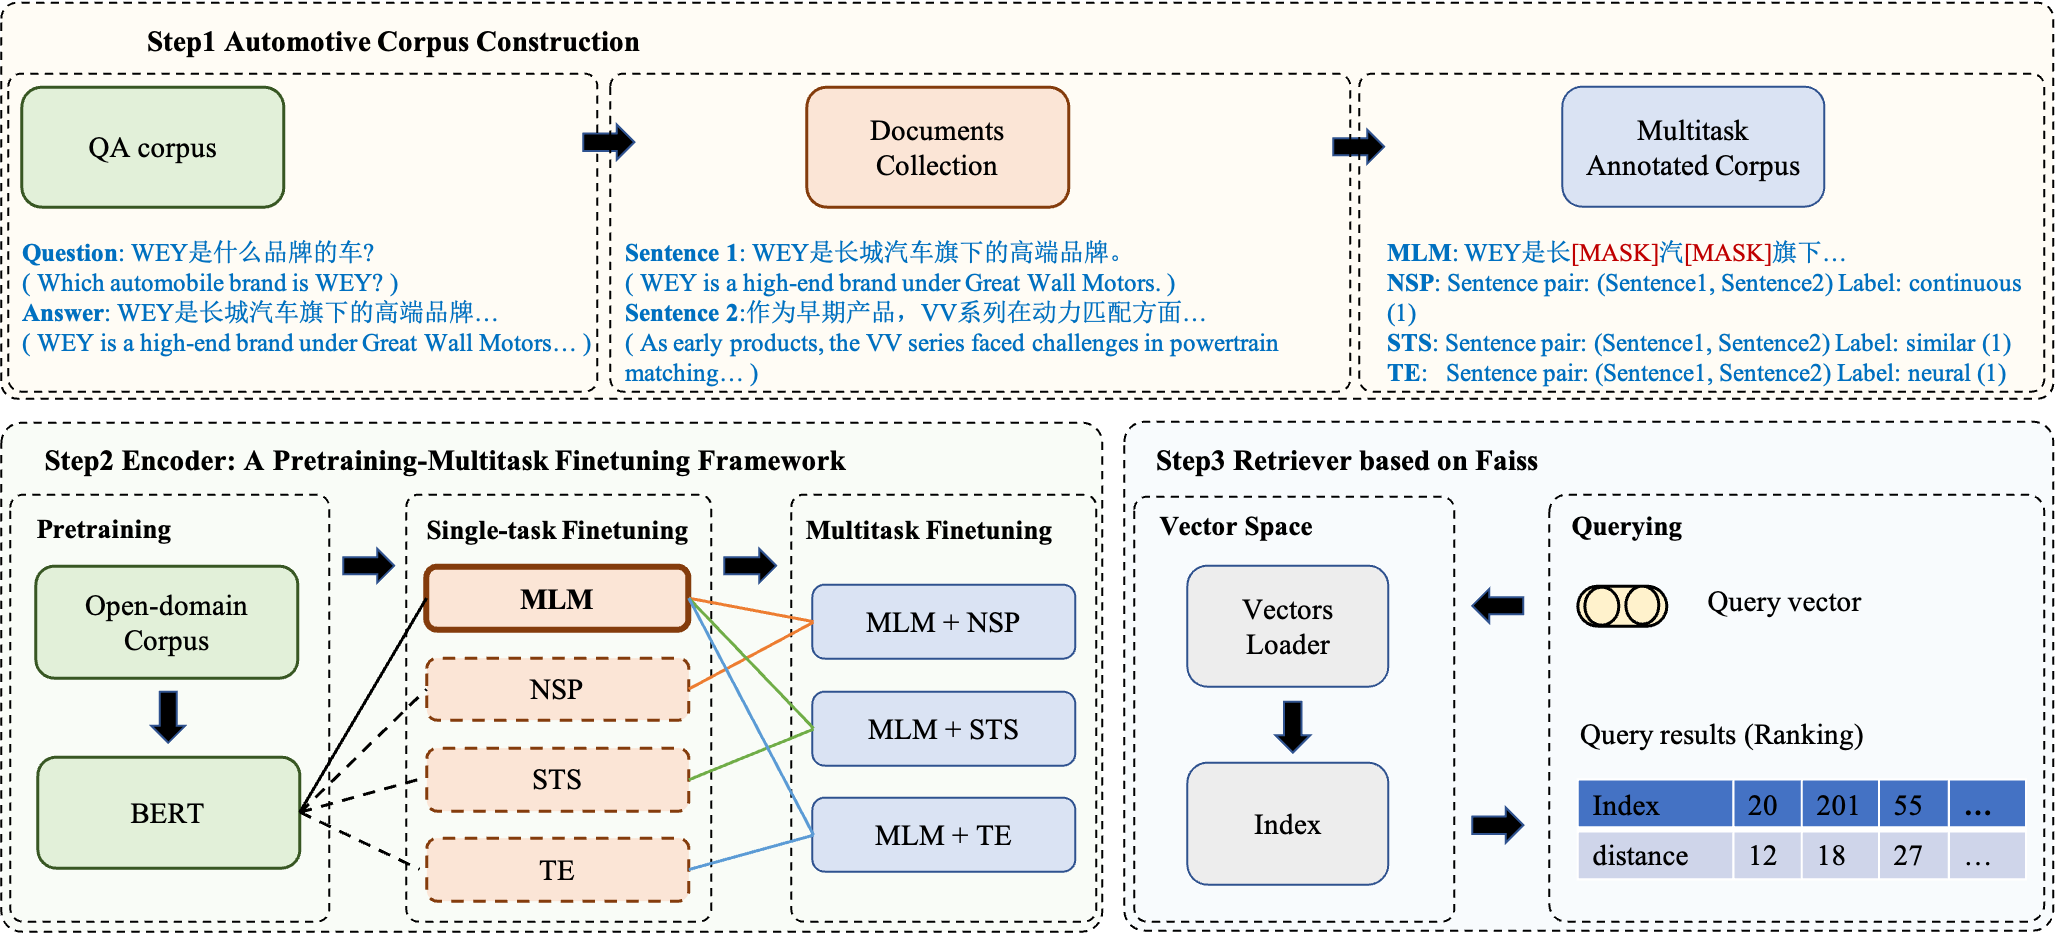
\includegraphics[width=14.0cm]{overview}
	\caption{An overview of our retrieval-based QA system. \textbf{(a) Step 1}: Automotive Corpus Construction. \textbf{(b) Step 2}: The encoder module under a pretraining-multitask fine-tuning framework. \textbf{(c) Step 3}: The retriever module based on Faiss library.}
	\label{fig:overview}
\end{figure}   
\unskip

\subsection{Corpus Construction}
\label{sec:corpus_construction}
We construct a QA dataset specific to the automotive domain by gathering question-answer pairs from authoritative resources, including professional databases, websites and other relevant resources. This dataset comprises a total of 7,157 question-answer pairs, with each pair consisting of a question and its corresponding answer. \tableref{tab:base_corpus} provides an illustrative example of the dataset. 

\begin{table}[H] 
	\caption{The constructed Chinese QA corpus in automotive domain.} \label{tab:base_corpus}
	\newcolumntype{C}{>{\centering\arraybackslash}X}
	\begin{tabularx}{\textwidth}{C}
		\toprule
		\textbf{An Example of QA pairs}	\\
		\midrule
		\{ ``id'': 0,~~~~~~~~~~~~~~~~~~~~~~~~~~~~~~~~~~~~~~~~~~~~~~~~~~~~~~~~~~~~~~~~ \\
		``question'': ``WEY是什么品牌的车?'',~~~~~~~~~~~~~~~~~~~~~~ \\
		~~~~~~~~~~ ({\color{blue} Which automobile brand is WEY?}) \\ 
		``answer'': ``WEY是长城汽车旗下的高端品牌…'', ~~~~~~~\\
		 ~~~~~~~~~~~~~~~~~~~~~~~~~~~~~~~~~~({\color{blue} WEY is a high-end brand under Great Wall Motors…}) \\
		\}~~~~~~~~~~~~~~~~~~~~~~~~~~~~~~~~~~~~~~~~~~~~~~~~~~~~~~~~~~~~~~~~~~~~~~~~~\\
%		\midrule
%		Entry 1		\\
%		Entry 2	Dat \textsuperscript{1}\\
		\bottomrule
	\end{tabularx}
%	\noindent{\footnotesize{\textsuperscript{1} Tables may have a footer.}}
\end{table}


\begin{table}[H] 
	\caption{The constructed Chinese QA corpus in automotive domain.} \label{tab:annotated_corpus}
	\newcolumntype{C}{>{\centering\arraybackslash}X}
	\begin{tabularx}{\textwidth}{p{2cm}L} 
		\toprule
		\textbf{Name}  & \textbf{Data Format}	\\
		\midrule
		MLM Corpus  & \textbf{[MASK][MASK]}车队首次在1994年的JGTC第四站比\textbf{[MASK]}中亮相,获得了资格赛第二名的位置。{\color{blue} (The [MASK] team made its debut in the fourth round of the JGTC  in 1994, securing the second position in the qualifying [MASK].) } \\
		\midrule
		NSP Corpus  & \textbf{Sentence1}: 上世纪90年代,TRD为丰田TOM'S车队打造了Supra赛车。{\color{blue} (In the 1990s, TRD built Supra race cars for the Toyota TOM'S team.) }
		\textbf{Sentence2}: 丰田车队首次在1994年的JGTC第四站比赛中亮相,获得了资格赛第二名的位置。{\color{blue} (The Toyota team made its debut in the fourth round of the JGTC  in 1994, securing the second position in the qualifying race.)} ~~~~~~~~~~~~~~~~~~~~~~~~~~~~~~~~\textbf{Label}: continuous (1)\\
		\midrule
		STS Corpus & \textbf{Sentence1}: 丰田车队首次在1994年的JGTC第四站比赛中亮相,获得了资格赛第二名的位置。{\color{blue} (The Toyota team made its debut in the fourth round of the JGTC  in 1994, securing the second position in the qualifying race.)}
		\textbf{Sentence2}: 在1994年的JGTC第四站比赛中,丰田车队首次参赛,并在资格赛中获得了第二名的成绩。{\color{blue} (In 1994, during the fourth round of the JGTC, the Toyota team made its debut and secured a second-place finish in the qualifying race.)} ~~~~~~~~~~~~~~~~~~~~~~~~~~~~~~~~~~~~~~~~~~~~~~~~~~~~~~~~~~~~~~~~~~~~~~~~~ \textbf{Label}: similar (1) ~~~~~~~~		\\
		\midrule
		TE Corpus  &  \textbf{Sentence1}: 一个年轻的黑人正试图向另外两个人解释一些事情。{\color{blue} (A young black person is trying to explain something to two other individuals.)}
		\textbf{Sentence2}: 一位年轻的黑人男子正在和另外两位说话。{\color{blue} (A young black man is talking to two other people.)} ~~~~~~~~~~~~~~~~~~~~~~~~~~~~~~~~~~~~~~~~~~~~~~~~~~~~~~~~~~~~~ \textbf{Label}: entailment (0) ~~~~~		\\
		\bottomrule
	\end{tabularx}
	%	\noindent{\footnotesize{\textsuperscript{1} Tables may have a footer.}}
\end{table}

\section{Experiments}
In this section, we first create an evaluation dataset for the automotive domain. Next, we introduce evaluation metrics utilized in our experiments. Finally, we conduct a comparative analysis against competing models to substantiate the effectiveness of our system.

\subsection{Evaluation Dataset}
Firstly, we create a retrieval corpus (shown in \tableref{tab:question_set}) utilizing the question set outlined  in \secref{sec:corpus_construction}. 
Then, we randomly sample 100 questions from the retrieval corpus. These selected questions are then subjected to synonymous rephrasing using ChatGPT, which ultimately leads to the creation of the evaluation dataset (shown in \tableref{tab:eval_dataset}).

\begin{table}[H] 
	\caption{The retrieval corpus consisted of all questions in QA dataset.} \label{tab:question_set}
	\newcolumntype{C}{>{\centering\arraybackslash}X}
	\begin{tabularx}{\textwidth}{C}
		\toprule
		\textbf{Questions}	\\
		\midrule
		\{ 未来车门会是什么样?\} \\({\color{blue} What will the car doors of the future look like?})\\
		\midrule
		\{ WEY是什么品牌的车?\} \\({\color{blue} Which automobile brand is WEY?}) \\ \midrule
		\{ 长安沃尔沃和吉利沃尔沃有什么区别?\} \\ ({\color{blue} What is the difference between Changan Volvo and Geely Volvo?})\\
		%		\midrule
		%		Entry 1		\\
		%		Entry 2	Dat \textsuperscript{1}\\
		\bottomrule
	\end{tabularx}
	%	\noindent{\footnotesize{\textsuperscript{1} Tables may have a footer.}}
\end{table}

Specifically, we transform the rephrasing task description and the question text into prompts, which are fed into ChatGPT to generate the rephrased results. These results are then subject to manual screening to create the final evaluation dataset. The prompts are designed following specific principles: (1) Role assignment: ChatGPT assumes the role of an automotive engineer, for instance, with a prompt like ``Imagine you are an automotive engineer''. (2) Rephrasing task description: a detailed explanation of the rephrasing task requirements is provided, such as ``You will receive a text related to the automotive domain and your task is to rewrite it, ensuring that the length remains similar to the original while preserving its meaning''. (3) Result requirements: the desired outcomes of ChatGPT's generation are described, for example, with a prompt like ``Please provide 6 rephrased results for each data point and rank them in descending order based on their quality''. Subsequently, human annotators manually review the rephrased results generated by ChatGPT, carefully examining each question's rephrased versions, and selecting the top 4 synonyms with the highest quality. This process yields a dataset comprising 400 user queries, as depicted in Table 4. Each query corresponds to a question in the {\em queries} field and has a corresponding reference question in the retrieval corpus, indicated by the {\em reference} field. This user query dataset is utilized to evaluate the performance of the retrieval-based question answering model.

\begin{table}[H] 
	\caption{The evaluation dataset in our experiments.} \label{tab:eval_dataset}
	\newcolumntype{C}{>{\centering\arraybackslash}X}
	\begin{tabularx}{\textwidth}{L}
	\toprule
		\textbf{An illustration Example}	\\
		\midrule
		\{ ``reference'': ``长安cs75plus车型热销背后的几点思考'',~~~~~~~~~~~~~~~~~~~~~~~~~~~~~~~ \\
		~~~~~~~~~~~~~~~~~~~({\color{blue} Some thoughts behind the hot sales of the Changan CS75 Plus model.}) \\ 
		~~~``queries'': [\\
		~~~~~~``长安cs75plus车型热销背后原因解析'', \\
		~~~~~~~({\color{blue} Analysis of the reasons behind the high sales of the Changan CS75 Plus model.}) \\ 
		~~~~~~``购买长安cs75plus车型的几点原因'', \\
		~~~~~~ ({\color{blue} Several reasons for purchasing the Changan CS75 Plus model.}) \\ 
		~~~~~~``长安cs75plus车型为什么能够热销,列出几点原因'', \\
		~~~~~~~({\color{blue} Please list a few reasons to explain why the Changan CS75 Plus model sells well.}) \\ 
		~~~~~~~``长安cs75plus车型,热销背后的原因思考'',~~~~ \\
		~~~~~~ ({\color{blue} Reflection on the reasons behind the popularity of the Changan CS75 Plus model.}) \\ 
		~~~~] ~~~~~~~~~~~~~~~~~~~~~~~~~~~\\
		\}~~~~~~~~~~~~~~~~~~~~~~~~~~~~~~~~~~~~~~~~~~~~~~~~~~~~~~~~~~~~~~~~~~~~~~~~~\\
		\bottomrule
	\end{tabularx}
	%	\noindent{\footnotesize{\textsuperscript{1} Tables may have a footer.}}
\end{table}


\subsection{Evaluation Metrics}
\label{sec:metrics}
The hit rate at K (Hit@K) is a widely used evaluation metric for assessing the performance of retrieval systems. It measures the capability to rank the correct target of user queries among the top K retrieval results. When conducting Hit@K for evaluation, a query is considered a hit if the true target is included in the top K retrieval results; otherwise, it is categorized as a miss. In our experiments, we utilize Hit@1, Hit@3, and Hit@5 as evaluation metrics for the retrieval model. Formally, the Hit@K is computed as:
\begin{linenomath}
	\begin{equation}\label{eq:hit}
		Hit@K = \frac{N_K}{|\mathcal{Q}|}, 
	\end{equation}
\end{linenomath}
where $N_K$ represents the total number of hits for $N$ retrieval tasks, and $|\mathcal{Q}|$ is the total number of true targets across all queries.

While Hit@K is a straightforward metric, it solely focuses on the top-ranked results, disregarding other potentially valuable outcomes. To account for the ranking of all results, we utilize the Mean Reciprocal Rank (MRR) as an evaluation metric. MRR is computed as follows:
\begin{linenomath}
	\begin{equation}\label{eq:mrr}
		MRR = \frac{1}{|S|}\sum_{i=1}^{|S|}\frac{1}{r_i}, 
	\end{equation}
\end{linenomath}
where $|S|$ represents the total number of queries, and $r_i$ denotes the ranking of the true target corresponding to the $i$-th query in the retrieved  results.

In addition, we present a novel evaluation metric designed based on real user behavior. Considering that the result page of the QA system  has the capability to display multiple results, the difference between the top-ranked and fifth-ranked feedback results holds minimal significance in terms of user experience. However, the MRR metric assigns a score difference of 0.8 between the first and fifth ranks (with a maximum score of 1). 
Moreover, considering that users typically limit their exploration to the initial pages of retrieval results, if a rank exceeds a certain threshold, it indicates a failure of the query sample to produce the correct result within the system. Despite a low ranking, MRR still provides a positive evaluation score when used for assessment. To address these concerns, we propose a new evaluation metric called Mean Linear Window Rank (MLWR). MLWR linearly adjusts the impact of ranking on the evaluation metric and incorporates a window size to exclude query samples with rankings beyond the predefined window. This approach better aligns with the user experience requirements of the system and provides a comprehensive assessment of retrieval system performance. Formally, MLWR is computed as follows:
\begin{linenomath}
	\begin{equation}\label{eq:mlwr}
		MLWR = \sum_{i=1}^{|S|}\frac{\max\{0, N-r_i+1\}}{N\times |S|}, 
	\end{equation}
\end{linenomath}
where $|S|$ represents the total number of samples, $r_i$ denotes the ranking of the true target corresponding to the $i$-th query in the retrieved  results, and $N$ is the window size. 

\subsection{Comparison Results}

In this section, we compare the performance of pretrained models, single-task fine-tuned models, and multitask fine-tuned models on the automotive domain QA retrieval task. By thoroughly examining the experimental results, we identify the most effective multitask fine-tuning strategy.


\begin{table}[H] 
	\caption{Comparison of Hit@K, MRR, MLWR using single-task fine-tuning models based on $\text{BERT}_{base}$.} \label{tab:single}
	\newcolumntype{C}{>{\centering\arraybackslash}X}
	\begin{tabularx}{\textwidth}{p{1.5cm}CCCCCCCCCC}
		\toprule
		\multirow{2}{*}{\textbf{Model}} & \multicolumn{2}{c}{Hit@1(\%)} & \multicolumn{2}{c}{Hit@3(\%)} & \multicolumn{2}{c}{Hit@5(\%)} & \multicolumn{2}{c}{MRR(\%)} & \multicolumn{2}{c}{MLWR(\%)} \\
		\cline{2-11} 
		\addlinespace
		& CLS           & MEAN          & CLS           & MEAN          & CLS           & MEAN          & CLS          & MEAN         & CLS           & MEAN         \\
		\midrule
		$\text{BERT}_{base}$   & 30.00         & 64.50         & 39.50         & 72.25         & 43.25         & 77.25         & 36.57        & 70.21        & 47.37         & 79.97   \\ 
%		BERT   & 30.00         & 64.50         & 39.50         & 72.25         & 43.25         & 77.25         & 36.57        & 70.21        & 47.37         & 79.97        \\
		FT-MLM & 47.25         & 77.00         & 55.50         & 83.50         & 57.00         & 85.75         & 52.19        & 80.94        & 58.96         & 86.76        \\
		FT-STS & 13.00         & 60.25         & 18.50         & 71.25         & 22.25         & 74.75         & 17.73        & 66.58        & 26.21         & 76.19        \\
		FT-TE  & 5.00          & 24.75         & 8.50          & 30.25         & 9.00          & 32.75         & 7.27         & 28.89        & 10.73         & 35.41        \\
		FT-NSP & 14.75         & 59.00         & 14.75         & 67.75         & 20.75         & 71.00         & 18.53        & 64.53        & 24.56         & 73.29  \\ 
%		$\text{BERT}_{large}$   & 26.50         & 64.50         & 39.50         & 72.25         & 43.25         & 77.25         & 36.57        & 70.21        & 47.37         & 79.97   \\ 
		\bottomrule
	\end{tabularx}
	%	\noindent{\footnotesize{\textsuperscript{1} Tables may have a footer.}}
\end{table}



\begin{table}[H] 
	\caption{Comparison of Hit@K, MRR, MLWR using multitask fine-tuning models based on $\text{BERT}_{base}$.} \label{tab:multi}
	\newcolumntype{C}{>{\centering\arraybackslash}X}
	\begin{tabularx}{\textwidth}{p{3.0cm}CCCCCC}
	\toprule
	\multicolumn{1}{c}{Model}                & Hit@1(\%) & Hit@3(\%) & Hit@5(\%) & MRR(\%) & MLWR(\%) \\
	\midrule
	STS+MLM {[}CLS{]}  & 74.25     & 84.00     & 85.25     & 79.54   & 87.12    \\
	NSP+MLM {[}CLS{]}  & 8.25      & 15.00     & 18.75     & 13.08   & 21.65    \\
	STS+MLM {[}MEAN{]} & 77.50     & 84.75     & 87.00     & 81.60   & 87.71    \\
	NSP+MLM {[}MEAN{]} & 73.25     & 78.75     & 80.50     & 76.77   & 82.17   \\
	\bottomrule
	\end{tabularx}
	%	\noindent{\footnotesize{\textsuperscript{1} Tables may have a footer.}}
\end{table}

\begin{table}[H] 
	\caption{Comparison of Hit@K, MRR, MLWR using the best single-task and multitask fine-tuning models based on $\text{BERT}_{large}$ and $\text{RoBERTa}$.} \label{tab:sup}
	\newcolumntype{C}{>{\centering\arraybackslash}X}
	\begin{tabularx}{\textwidth}{p{1.5cm}CCCCCCCCCC}
		\toprule
		\multirow{2}{*}{\textbf{Model}} & \multicolumn{2}{c}{Hit@1(\%)} & \multicolumn{2}{c}{Hit@3(\%)} & \multicolumn{2}{c}{Hit@5(\%)} & \multicolumn{2}{c}{MRR(\%)} & \multicolumn{2}{c}{MLWR(\%)} \\
		\cline{2-11} 
		\addlinespace
		& CLS           & MEAN          & CLS           & MEAN          & CLS           & MEAN          & CLS          & MEAN         & CLS           & MEAN         \\
		\toprule
		$\text{BERT}_{large}$   & 26.50         & 64.50         & 39.50         & 72.25         & 43.25         & 77.25         & 36.57        & 70.21        & 47.37         & 79.97   \\ 
		FT-MLM & 29.25         & 76.75         & 36.50         & 82.00         & 39.50         & 85.25        & 33.88        & 80.42        & 41.56        & 86.19        \\
		MLM+STS & 18.50        & 78.00        & 22.20         & 83.50        & 23.50         & 85.75         & 21.13       & 81.67     & 25.16       & 88.42      \\ \toprule[0.2mm]
		$\text{RoBERTa}$   & 69.00         & 73.00         & 77.75      & 79.50        & 79.25        & 82.75        & 74.16        & 77.41       & 81.59         & 84.61   \\ 
		FT-MLM & 73.25        & 75.75        & 79.25        & 81.75        & 83.25         & 84.00         &  77.63        & 79.79        & 85.31         & 86.81        \\
		MLM+STS & 37.50         & 78.75        & 48.25         & 84.50       & 51.75        & 87.75         & 44.46     & 82.50       & 55.16         & 88.79       \\
		\bottomrule[0.2mm]
	\end{tabularx}
	%	\noindent{\footnotesize{\textsuperscript{1} Tables may have a footer.}}
\end{table}


To illustrate the generalization capability of our framework in mitigating bias within pretrained models, we extend our evaluation beyond the BERT-base model to also include the BERT-large and RoBERTa models. As shown in \tableref{tab:sup}, our framework exhibits effective generalization   across a variety of pretrained models. It is worth nothing that RoBERTa, which is solely pretrained using the MLM task, demonstrates good performance with the CLS encoding, achieving a Hit@1 score of 69\%. However, in pretraining models such as BERT-base and BERT-large, the CLS representation primarily learns from the NSP task, resulting in sub-optimal performance when directly utilizing the  CLS encoding. These findings highlight the negative impact of the NSP task as a training objective on QA tasks, while emphasizing the benefits of the MLM task as a training objective for downstream QA tasks. 

%Furthermore, in order to showcase the effectiveness of the retriever module in our proposed system, we compare its performance using different indexing structures as described in Section 3.2. Specifically, we evaluate the retriever module using brute force, IndexPQ index, IndexHNSWFlat, and IndexFlatL2. 
%As shown in 
\subsection{Case Study}
In this section,  we conduct a case study to qualitatively analyze competing models. 
\tableref{tab:case} presents the results obtained when inputting an example user query, 
namely ``如何对高尔夫7系列车型进行自我检修?'' ({\color{blue} How to perform self-maintenance on Volkswagen Golf7 series?}), and showcases the responses retrieved by the competing models utilizing $\text{BERT}_{base}$ in proposed framework.
The baseline BERT model provides a historical overview of the 7th Generation Volkswagen Golf, while the single-task FT-MLM model compares the 308S and Golf 7 models. However, neither of these models is capable of providing an accurate answer to the query. In contrast, the STS+MLM joint fine-tuning model effectively responds with the precise and specific steps to perform maintenance on the FAW-Volkswagen Golf7, thereby correctly addressing the query.
The STS+MLM joint model demonstrates its effectiveness in capturing the query intentions, surpassing other competing models in terms of qualitative performance.


\begin{table}[H] 
	\caption{Retrieved answers from baseline $\text{BERT}_{base}$ model, single-task FT-MLM model, and multitask STS+MLM model.} \label{tab:case}
	\newcolumntype{C}{>{\centering\arraybackslash}X}
	\begin{tabularx}{\textwidth}{cp{10cm}}
		\toprule
		\multicolumn{2}{p{12cm}}{\hangindent=2.2cm \hangafter=1 \textbf{Input Query}: ``如何对高尔夫7系列车型进行自我检修?'' ({\color{blue} How to perform self-maintenance on Volkswagen Golf7 series?})}   \\
		\midrule
		\textbf{Model} & \textbf{Retrieved answers} \\ \midrule
		$\text{BERT}_{base}$  &  1. 高尔夫Mk1:1974年5月,第一代高尔夫... 2. 高尔夫Mk2:1983年8月,大众推出第二代... ({\color{blue} 1. Golf Mk1: In May 1974, the first generation Golf was introduced..  2. Golf Mk2: In August 1983, Volkswagen unveiled the second generation...})  \\\midrule
		FT-MTM  &       1. 动力组合对比:高尔夫一共有三种排量...	 2. 质保政策对比:高尔夫官方保修周期为3年或者...
		  ({\color{blue} 1. Powertrain Comparison: The Golf is available in three different engine displacements... 2. Warranty Policy Comparison: The official warranty period for the Golf is 3 years or...})   \\ \midrule
		MLM+STS  &   1. 更换4.5升5w40美孚全合成机油、博世机滤、博世空气滤芯、博世空调滤芯、博世汽油滤芯、3m燃油添加剂、免拆三元催化清洗剂
2. 动平衡、更换原厂轮毂盖
		 ({\color{blue} 1. Replace 4.5 liters of 5w40 Mobil fully synthetic engine oil, Bosch oil filter, Bosch air filter, Bosch cabin air filter, Bosch fuel filter, 3M fuel additive, and non-dismantle catalytic converter cleaner.  2. Dynamic balancing and replace original wheel hub covers. }) \\
		\bottomrule
	\end{tabularx}
	%	\noindent{\footnotesize{\textsuperscript{1} Tables may have a footer.}}
\end{table}


\section{Conclusion}
In this paper, we first focus on constructing QA corpora, document sets, and multitask fine-tuning datasets specifically tailored to the automotive domain. Then, we propose a pretraining-multitask fine-tuning learning framework to develop an encoder model that incorporates domain knowledge, enhancing the semantic representation of texts and enabling effective retrieval QA applications. The experimental results reveal that within the multitask fine-tuning framework (based on $\text{BERT}_{base}$), the joint fine-tuned model MLM+STS achieves the highest performance. It attains Hit@1 and Hit@3 accuracies of 77.5\% and 84.75\%, respectively, along with an MLWR of 87.71\%. These outcomes signify substantial improvements of 12.5, 12.5, and 28.16 percentage points, respectively, compared to the baseline BERT model. Additionally, when compared to the best-performing single-task fine-tuned model, FT-MLM, the observed enhancements amount to 0.5, 1.25, and 0.95 percentage points, respectively.

%All figures and tables should be cited in the main text as Figure~\ref{fig1}, Table~\ref{tab1}, etc.

%\section{Discussion}
%
%Authors should discuss the results and how they can be interpreted from the perspective of previous studies and of the working hypotheses. The findings and their implications should be discussed in the broadest context possible. Future research directions may also be highlighted.

%%%%%%%%%%%%%%%%%%%%%%%%%%%%%%%%%%%%%%%%%%
%\section{Conclusions}
%
%This section is not mandatory, but can be added to the manuscript if the discussion is unusually long or complex.


%%%%%%%%%%%%%%%%%%%%%%%%%%%%%%%%%%%%%%%%%%
\vspace{6pt} 

%%%%%%%%%%%%%%%%%%%%%%%%%%%%%%%%%%%%%%%%%%
%% optional
%\supplementary{The following supporting information can be downloaded at:  \linksupplementary{s1}, Figure S1: title; Table S1: title; Video S1: title.}

% Only for journal Methods and Protocols:
% If you wish to submit a video article, please do so with any other supplementary material.
% \supplementary{The following supporting information can be downloaded at: \linksupplementary{s1}, Figure S1: title; Table S1: title; Video S1: title. A supporting video article is available at doi: link.}

% Only for journal Hardware:
% If you wish to submit a video article, please do so with any other supplementary material.
% \supplementary{The following supporting information can be downloaded at: \linksupplementary{s1}, Figure S1: title; Table S1: title; Video S1: title.\vspace{6pt}\\
%\begin{tabularx}{\textwidth}{lll}
%\toprule
%\textbf{Name} & \textbf{Type} & \textbf{Description} \\
%\midrule
%S1 & Python script (.py) & Script of python source code used in XX \\
%S2 & Text (.txt) & Script of modelling code used to make Figure X \\
%S3 & Text (.txt) & Raw data from experiment X \\
%S4 & Video (.mp4) & Video demonstrating the hardware in use \\
%... & ... & ... \\
%\bottomrule
%\end{tabularx}
%}

%%%%%%%%%%%%%%%%%%%%%%%%%%%%%%%%%%%%%%%%%%
%\authorcontributions{For research articles with several authors, a short paragraph specifying their individual contributions must be provided. The following statements should be used ``Conceptualization, X.X. and Y.Y.; methodology, X.X.; software, X.X.; validation, X.X., Y.Y. and Z.Z.; formal analysis, X.X.; investigation, X.X.; resources, X.X.; data curation, X.X.; writing---original draft preparation, X.X.; writing---review and editing, X.X.; visualization, X.X.; supervision, X.X.; project administration, X.X.; funding acquisition, Y.Y. All authors have read and agreed to the published version of the manuscript.'', please turn to the  \href{http://img.mdpi.org/data/contributor-role-instruction.pdf}{CRediT taxonomy} for the term explanation. Authorship must be limited to those who have contributed substantially to the work~reported.}

\funding{ This research was supported by the Natural Science Foundation of Zhejiang Province, China (Grant No. LQ22F020027) and the Key Research and Development Program of Zhejiang Province, China (2023C01041).}


%\acknowledgments{In this section you can acknowledge any support given which is not covered by the author contribution or funding sections. This may include administrative and technical support, or donations in kind (e.g., materials used for experiments).}

\conflictsofinterest{The authors declare no conflict of interest.} 

%%%%%%%%%%%%%%%%%%%%%%%%%%%%%%%%%%%%%%%%%%


%% Only for journal Encyclopedia
%\entrylink{The Link to this entry published on the encyclopedia platform.}



%%%%%%%%%%%%%%%%%%%%%%%%%%%%%%%%%%%%%%%%%%
\begin{adjustwidth}{-\extralength}{0cm}
%\printendnotes[custom] % Un-comment to print a list of endnotes

\reftitle{References}

% Please provide either the correct journal abbreviation (e.g. according to the “List of Title Word Abbreviations” http://www.issn.org/services/online-services/access-to-the-ltwa/) or the full name of the journal.
% Citations and References in Supplementary files are permitted provided that they also appear in the reference list here. 

%=====================================
% References, variant A: external bibliography
%=====================================
%\bibliography{your_external_BibTeX_file}

%=====================================
% References, variant B: internal bibliography
%=====================================
\begin{thebibliography}{999}
	% Reference 1
	\bibitem[Gupta(2005)]{asq-system}
	Gupta, N.; Tur, G.; Hakkani-Tur, D.; et al. The AT\&T spoken language understanding system. {\em IEEE Transactions on Audio, Speech, and Language Processing}, {\bf 2005}, {\em 14(1)}, 213-222.
	\bibitem[Ferrucci(2010)]{watson}
	Ferrucci, D.G.; Brown, E.; Chu-Carroll, J.; Fan, J.; Gondek, D.; Kalyanpur, A.A.; Lally, A.; Murdock, J.W.; Nyberg, E.; Prager, J.; Schlaefer, N.; Welty, C. Building Watson: An Overview of the DeepQA Project. {\em AI Magazine} {\bf 2010}, {\em 31(3)}, 59--79.
	\bibitem[Qu(2018)]{odqa2018}
	Qu, C.; Yang, L.; Qiu, M.H. Open domain question answering using early fusion of knowledge bases and text. Available online: https://doi.org/10.48550/arXiv.1809.00782. (accessed on 19-05-2023).
	\bibitem[Vaswani(2017)]{transformers2017}
	Vaswani, A.; Shazeer, N.; Parmar, N.; Uszkoreit, J.; Jones, L.; Gomez, A.N.; Polosukhin, I. Attention Is All You Need. In Proceedings of Advances in Neural Information Processing Systems(ANIPS), California, USA, 2017; 5998-6008.
	\bibitem[Devlin(2019)]{bert2019}
	Devlin, J.; Chang, M.W.; Lee, K.; Toutanova, K. BERT: Pre-training of Deep Bidirectional Transformers for Language Understanding. In Proceedings of the Conference of the North American Chapter of the Association for Computational Linguistics: Human Language Technologies (NAACL-HLT), Minneapolis, 2019; 4171-4186.
	\bibitem[Radford(2018)]{gpt}
	Radford, A.; Narasimhan, K.; Salimans, T.; Sutskever, I. Improving Language Understanding by Generative Pre-Training. Available online: https://cdn.openai.com/research-covers/language-unsupervised/language\_understanding\_paper.pdf. (accessed on 19-05-2023).
	\bibitem[Radford(2020)]{gpt2}
	Radford, A.; Wu, J.; Child, R.; Luan, D.; Amodei, D.; Sutskever, I. Language Models are Unsupervised Multitask Learners. Available online: https://cdn.openai.com/better-language-models/language\_models\_are\_unsupervised\_multitask\_learners.\\pdf. (accessed on 19-05-2023).
	\bibitem[Brown(2020)]{gpt3}
	Brown, T.; Mann, B.; Ryder, N.; et al. Language models are few-shot learners. In proceedings of Advances in Neural Information Processing Systems, Virtual-only Conference, 2020, 33: 1877-1901.
	\bibitem[Rajpurkar(2016)]{squad}
	Rajpurkar, P.; Zhang, J.; Lopyrev, K.; Liang, P. Squad: 100,000+ questions for machine comprehension of text. In Proceedings of the Conference on Empirical Methods in Natural Language Processing(EMNLP), Austin, Texas, USA, 2016, 2383-2392.
	\bibitem[Rajpurkar(2018)]{squad2.0}
	Rajpurkar, P.; Jia, R.; Liang, P. Know what you don’t know: Unanswerable questions for squad. In Proceedings of the 56th Annual Meeting of the Association for Computational Linguistics (Volume 2: Short Papers), Melbourne, Australia, 2018, 784–789.
	\bibitem[Li(2022)]{multispanqa}
	Li, H.; Tomko, M.; Vasardani, M.; Baldwin, T. MultiSpanQA: A dataset for multi-span question answering. In Proceedings of the Conference of the North American Chapter of the Association for Computational Linguistics: Human Language Technologies (NAACL-HLT), Seattle, Washington, 2022, 1250–1260.
	\bibitem[Yang(2019)]{bertserini}
	Yang, Wei; et al. End-to-end open-domain question answering with bertserini. Available online: https://doi.org/10.48550/ar-\\Xiv.1902.01718. (accessed on 19-05-2023).
	\bibitem[Zhang(2022)]{qa-survey}
	Zhang, Q.; Chen, S.S.; Xu, D.K.; Cao, Q.Q.; Chen, X.J.; Cohn, T.; Fang, M. A Survey for Efficient Open Domain Question Answering. Available Online: https://arxiv.org/abs/2211.07886. (accessed on 19-05-2023).
	\bibitem[Jones(1972)]{tf-idf}
	Jones, S.K. A statistical interpretation of term specificity and its application in retrieval. {\em Journal of Documentation} {\bf 1972}, {\em 28(1)}, 11--21.
%	\bibitem[Lin(2017)]{multichannel}
%	Lin, B. Y.; Xu, F. F.; Luo, Z.; et al. Multi-channel bilstm-crf model for emerging named entity recognition in social media. In Proceedings of the 3rd Workshop on Noisy User-generated Text, Copenhagen, Denmark, 2017, 160-165.
	\bibitem[Baldwin(2015)]{hand-crafted-features}
	Baldwin, T.; Marneffe M.C.; Han, B.; et al. Shared tasks of the 2015 workshop on noisy user-generated text: Twitter lexical normalization and named entity recognition. In Proceedings of the workshop on noisy user-generated text, Beijing, China, 2015, 126-135.
	\bibitem[Derczynski(2015)]{tweet}
	Derczynski, L.; Maynard, D.; Rizzo, G.; et al. Analysis of named entity recognition and linking for tweets. {\em Information Processing \& Management} {\bf 2015}, {\em 51(2)}, 32-49.
	\bibitem[Mikolov(2013)]{word2vec}
	Mikolov, T.; Chen, K.; Corrado, G.; Dean, J. Efficient estimation of word representations in vector space. Available online: https://arxiv.org/abs/1301.3781. (accessed on 19-05-2023).
%	\bibitem[Le(2014)]{word2vec2}
%	Le, Q.; Mikolov, T. Distributed representations of sentences and documents. In Proceedings of the 31st International Conference on Machine Learning (ICML), Beijing, China, 2014; 1188-1196.
	\bibitem[Harris(1954)]{distributed-hypothesis}
	Harris, Z.S. Distributional structure. {\em Journal of Documentation} {\bf 1954}, {\em 10(2-3)}, 146--162.
	\bibitem[Le(2014)]{glove}
	Pennington, J.; Socher, R.; Manning, C.D. GloVe: Global Vectors for Word Representation. In Proceedings of the 2014 conference on empirical methods in natural language processing (EMNLP),  Maryland, USA, 2014; 1532-1543.
	\bibitem[Vaswani(2017)]{cove}
	McCann, B.; Bradbury, J.; Xiong, C.; Socher, R. Learned in translation: Contextualized word vectors. In Proceedings of Advances in Neural Information Processing Systems(NIPS), California, USA, 2017; 6297-6308.
	\bibitem[Peters(2018)]{elmo}
	Peters, M.E.; Neumann, M.; Iyyer, M.; Gardner, M.; Clark, C.; Lee, K.; Zettlemoyer, L. Deep contextualized word representations. In Proceedings of the 2018 Conference of the North American Chapter of the Association for Computational Linguistics: Human Language Technologies, New Orleans, USA, 2018; 2227-2237.
	\bibitem[Devika(2021)]{app1}
	Devika, R.; Vairavasundaram, S.; Mahenthar, C.S.J.; et al. A Deep Learning Model Based on BERT and Sentence Transformer for Semantic Keyphrase Extraction on Big Social Data. In  IEEE Access \textbf{2021}, 9, 165252-165261.
	\bibitem[Natarajan(2022)]{app2}
	Natarajan, B.; Rajalakshmi, E.; Elakkiya, R; et al. Development of an End-to-End Deep Learning Framework for Sign Language Recognition, Translation, and Video Generation. In IEEE Access \textbf{2022}, 10, 104358-104374.
	\bibitem[Bentley(1975)]{kd-tree}
	Bentley, J.L. Multidimensional binary search trees used for associative searching. {\em Communications of the ACM} {\bf 1975}, {\em 18(9)}, 509-517.
	\bibitem[Liu(2006)]{ball-tree}
	Liu, T.; Moore, A.W.; Gray, A.; New algorithms for efficient high-dimensional nonparametric classification. {\em JMLR} {\bf 2006}, 7, 1135–1158.
	\bibitem[Omohundro(1989)]{ball-tree2}
	Omohundro SM. Five balltree construction algorithms. Berkeley, California, USA: International Computer Science Institute, 1989.
	\bibitem[Friedman(1977)]{knn-graph}
	Friedman, J.H.; Bentley, J.L.; Finkel, R.A. An algorithm for finding best matches in logarithmic expected time. {\em ACM Transactions on Mathematical Software} {\bf 1977}, {\em 3(3)}, 209-226.
	\bibitem[Jégou(2011)]{pq}
	Jégou, H.; Douze, M.; Schmid, C. Product quantization for nearest neighbor search. {\em IEEE Transactions on Pattern Analysis and Machine Intelligence} {\bf 2011}, {\em 33(1)}, 117-128.
	\bibitem[20Indyk(1998)]{lsh}
	Indyk, P.; Motwani, R. Approximate nearest neighbors: towards removing the curse of dimensionality. In Proceedings of the Thirtieth Annual ACM Symposium on Theory of Computing, New York, USA, 1998; 604-613.
	\bibitem[21Malkov(2018)]{hnsw}
	Malkov, Y.A.; Yashunin, D.A. Efficient and robust approximate nearest neighbor search using Hierarchical Navigable Small World graphs. Available online: https://arxiv.org/abs/1603.09320. (accessed on 19-05-2023).
	\bibitem[Jégou(2010)]{pns}
	Jégou, H.; Perronnin, F.; Douze, M.; Sánchez, J.; Pérez, P.; Schmid, C. Aggregating local descriptors into a compact image representation. In Proceedings of the 2010 IEEE Computer Society Conference on Computer Vision and Pattern Recognition, San Francisco, USA, 2010; 3304-3311.
	\bibitem[Wang(2019)]{haq}
	Wang, K.; Liu, Z.; Lin, Y.; Lin, W.; Han, S. HAQ: Hardware-Aware Automated Quantization with Mixed Precision. In Proceedings of  the IEEE Computer Society Conference on Computer Vision and Pattern Recognition, Los Angeles, USA, 2019; 1669-1678.	
	\bibitem[Johnson(2011)]{faiss}
	Johnson, J.; Douze, M.; Jégou, H. Billion-scale similarity search with GPUs. {\em IEEE Transactions on Big Data} {\bf 2019}, {\em 7(3)}, 535-547.	
%	\bibitem[Zhu(2015)]{}
%	Zhu, Y.K.; Kiros, R.; Zemel, R.; Salakhutdinov, R.; Urtasun, R.; Torralba, A.; Fidler, S. Aligning books and movies: Towards story-like visual explanations by watching movies and reading books. In Proceedings of the IEEE International Conference on Computer Vision, Santiago, Republic of Chile, 2015; 19-27.
	\bibitem[Liu(2019)]{roberta}
	Liu, Y.; Ott, M.; Goyal, N.; Du, J.; Joshi, M.; Chen, D. RoBERTa: A Robustly Optimized BERT Pretraining Approach. Available online: https://arxiv.org/abs/1603.09320. (accessed on 19-05-2023).
	\bibitem[Johnson(2020)]{spanbert}
	Clark, C.; Lee, K.; Chang, M.W.; Kwiatkowski, T.; Collins, M.; Toutanova, K. SpanBERT: Improving Pre-training by Representing and Predicting Spans. {\em Transactions of the Association for Computational Linguistics} {\bf 2020}, {\em 8}, 64-77.
	%	% Reference 2
%	\bibitem[Author2(year)]{ref-book1}
%	Author~2, L. The title of the cited contribution. In {\em The Book Title}; Editor 1, F., Editor 2, A., Eds.; Publishing House: City, Country, 2007; pp. 32--58.
%	% Reference 3
%	\bibitem[Author3(year)]{ref-book2}
%	Author 1, A.; Author 2, B. \textit{Book Title}, 3rd ed.; Publisher: Publisher Location, Country, 2008; pp. 154--196.
%	% Reference 4
%	\bibitem[Author4(year)]{ref-unpublish}
%	Author 1, A.B.; Author 2, C. Title of Unpublished Work. \textit{Abbreviated Journal Name} year, \textit{phrase indicating stage of publication (submitted; accepted; in press)}.
%	% Reference 5
%	\bibitem[Author5(year)]{ref-communication}
%	Author 1, A.B. (University, City, State, Country); Author 2, C. (Institute, City, State, Country). Personal communication, 2012.
%	% Reference 6
%	\bibitem[Author6(year)]{ref-proceeding}
%	Author 1, A.B.; Author 2, C.D.; Author 3, E.F. Title of presentation. In Proceedings of the Name of the Conference, Location of Conference, Country, Date of Conference (Day Month Year); Abstract Number (optional), Pagination (optional).
%	% Reference 7
%	\bibitem[Author7(year)]{ref-thesis}
%	Author 1, A.B. Title of Thesis. Level of Thesis, Degree-Granting University, Location of University, Date of Completion.
%	% Reference 8
%	\bibitem[Author8(year)]{ref-url}
%	Title of Site. Available online: URL (accessed on Day Month Year).
\end{thebibliography}
% Reference 2
%\bibitem[Author2(year)]{ref-book1}
%Author~2, L. The title of the cited contribution. In {\em The Book Title}; Editor 1, F., Editor 2, A., Eds.; Publishing House: City, Country, 2007; pp. 32--58.
%% Reference 3
%\bibitem[Author3(year)]{ref-book2}
%Author 1, A.; Author 2, B. \textit{Book Title}, 3rd ed.; Publisher: Publisher Location, Country, 2008; pp. 154--196.
%% Reference 4
%\bibitem[Author4(year)]{ref-unpublish}
%Author 1, A.B.; Author 2, C. Title of Unpublished Work. \textit{Abbreviated Journal Name} year, \textit{phrase indicating stage of publication (submitted; accepted; in press)}.
%% Reference 5
%\bibitem[Author5(year)]{ref-communication}
%Author 1, A.B. (University, City, State, Country); Author 2, C. (Institute, City, State, Country). Personal communication, 2012.
%% Reference 6
%\bibitem[Author6(year)]{ref-proceeding}
%Author 1, A.B.; Author 2, C.D.; Author 3, E.F. Title of presentation. In Proceedings of the Name of the Conference, Location of Conference, Country, Date of Conference (Day Month Year); Abstract Number (optional), Pagination (optional).
%% Reference 7
%\bibitem[Author7(year)]{ref-thesis}
%Author 1, A.B. Title of Thesis. Level of Thesis, Degree-Granting University, Location of University, Date of Completion.
%% Reference 8
%\bibitem[Author8(year)]{ref-url}
%Title of Site. Available online: URL (accessed on Day Month Year).

% If authors have biography, please use the format below
%\section*{Short Biography of Authors}
%\bio
%{\raisebox{-0.35cm}{\includegraphics[width=3.5cm,height=5.3cm,clip,keepaspectratio]{Definitions/author1.pdf}}}
%{\textbf{Firstname Lastname} Biography of first author}
%
%\bio
%{\raisebox{-0.35cm}{\includegraphics[width=3.5cm,height=5.3cm,clip,keepaspectratio]{Definitions/author2.jpg}}}
%{\textbf{Firstname Lastname} Biography of second author}

% For the MDPI journals use author-date citation, please follow the formatting guidelines on http://www.mdpi.com/authors/references
% To cite two works by the same author: \citeauthor{ref-journal-1a} (\citeyear{ref-journal-1a}, \citeyear{ref-journal-1b}). This produces: Whittaker (1967, 1975)
% To cite two works by the same author with specific pages: \citeauthor{ref-journal-3a} (\citeyear{ref-journal-3a}, p. 328; \citeyear{ref-journal-3b}, p.475). This produces: Wong (1999, p. 328; 2000, p. 475)




%%%%%%%%%%%%%%%%%%%%%%%%%%%%%%%%%%%%%%%%%%
%% for journal Sci
%\reviewreports{\\
%Reviewer 1 comments and authors’ response\\
%Reviewer 2 comments and authors’ response\\
%Reviewer 3 comments and authors’ response
%}
%%%%%%%%%%%%%%%%%%%%%%%%%%%%%%%%%%%%%%%%%%
\PublishersNote{}



\begin{table}[H] 
	\caption{Approach performance on complete MultiSpanQA valid set based on $\text{BERT}_{base}$.} \label{tab:single}
	\newcolumntype{C}{>{\centering\arraybackslash}X}
	\begin{tabularx}{\textwidth}{p{1.5cm}CCCCCCCC}
		\toprule
		\multirow{2}{*}{\textbf{Model}} & \multicolumn{3}{c}{Exact Match} & \multicolumn{3}{c}{Partial Match}  \\
		\cline{2-7} 
		\addlinespace
		& P           & R          & F           & P          & R           & F           \\
		\midrule
		Tase   & 60.28         & 55.59         & 65.83         & 78.16         & 78.27         & 78.06         \\ 
		Liquid & 61.44         & 58.39         & 64.84         & 78.56         & 78.65         & 78.46         \\
		C-rand & 63.05         & 58.51         & 68.34         & 79.42         & 78.70         & 80.14         \\
		ER-EEins  & 63.93          & 60.22         & 68.13          & 77.50         & 77.07          & 77.94         \\
		C-ER-EE & 62.90          & 61.02        & 64.89          & 76.72         & 78.56          & 74.97         \\
		Bagging & 64.44          & 61.63        & 67.50          & 79.52         & 80.49          & 78.57         \\
		\bottomrule
	\end{tabularx}
	%	\noindent{\footnotesize{\textsuperscript{1} Tables may have a footer.}}
\end{table}

\begin{table}[H] 
	\caption{Approach performance on complete MultiSpanQA valid set based on $\text{RoBERTa}_{base}$.} \label{tab:single}
	\newcolumntype{C}{>{\centering\arraybackslash}X}
	\begin{tabularx}{\textwidth}{p{1.5cm}CCCCCCC}
		\toprule
		\multirow{2}{*}{\textbf{Model}} & \multicolumn{3}{c}{Exact Match} & \multicolumn{3}{c}{Partial Match}  \\
		\cline{2-7} 
		\addlinespace
		& P & R & F & P & R & F \\
		\midrule
		Tase & 68.00 & 65.06 & 71.22 & 83.13 & 83.05 & 83.22 \\ 
		Liquid & 68.33 & 66.68 & 70.07 & 82.71 & 82.45 & 82.98 \\
		C-rand & 70.35 & 67.35 & 73.63 & 84.06 & 83.38 & 84.76 \\
		ER-EEins & 69.15 & 67.81 & 70.54 & 82.85 & 83.90 & 81.83 \\
		C-ER-EE & 70.44 & 67.813 & 73.26 & 82.80 & 82.45 & 83.15 \\
		Bagging & 70.86 & 69.03 & 72.79 & 84.82 & 85.53 & 84.12 \\
		\bottomrule
	\end{tabularx}
	%	\noindent{\footnotesize{\textsuperscript{1} Tables may have a footer.}}
\end{table}

\begin{table}[ht]
	\caption{Model performance on complete MultiSpanQA valid Subset with different answer types based on $\text{BERT}_{base}$.}
	\label{tab:single}
	\newcolumntype{C}{>{\centering\arraybackslash}X}
	\begin{tabularx}{\textwidth}{Cp{1.5cm}CCCCCCC}
		\toprule
		\multirow{2}{*}{\textbf{Type}} & \multirow{2}{*}{\textbf{Model}} & \multicolumn{3}{c}{Exact Match} & \multicolumn{3}{c}{Partial Match} \\
		\cmidrule{3-8} 
		& & P & R & F & P & R & F \\
		\midrule
		\multirow{6}{*}{DESC} & Tase & 32.76 & 27.33 & 40.87 & 64.46 & 68.61 & 60.79 \\ 
		& Liquid & 36.69 & 31.10 & 44.71 & 66.05 & 65.95 & 66.15 \\
		& C-rand & 38.74 & 32.89 & 47.12 & 68.31 & 70.32 & 66.42 \\
		& ER-EEins & 44.69 & 40.71 & 49.52 & 63.12 & 67.16 & 59.53 \\
		& C-ER-EE & 40.63 & 38.30 & 43.27 & 64.25 & 71.15 & 58.57 \\
		& Bagging & 39.91 & 36.69 & 43.75 & 66.70 & 73.68 & 60.93 \\
		\midrule
		\multirow{6}{*}{NUM} & Tase & 33.33 & 30.23 & 37.14 & 60.98 & 71.99 & 52.89 \\ 
		& Liquid & 34.33 & 31.25 & 38.10 & 60.68 & 68.15 & 54.69 \\
		& C-rand & 35.96 & 33.33 & 39.05 & 64.47 & 71.56 & 58.65 \\
		& ER-EEins & 36.20 & 34.48 & 38.10 & 59.02 & 65.63 & 53.62 \\
		& C-ER-EE & 36.71 & 37.25 & 36.19 & 57.09 & 69.04 & 48.67 \\
		& Bagging & 35.94 & 34.82 & 37.14 & 60.73 & 71.15 & 52.97 \\
		\midrule
		\multirow{6}{*}{HUM} & Tase & 70.68 & 67.64 & 74.00 & 83.09 & 83.93 & 82.28 \\ 
		& Liquid & 72.59 & 71.35 & 73.88 & 84.16 & 85.77 & 82.61 \\
		& C-rand & 73.80 & 71.17 & 76.63 & 84.36 & 85.30 & 83.43 \\
		& ER-EEins & 73.61 & 70.63 & 76.86 & 82.75 & 82.64 & 82.85 \\
		& C-ER-EE & 73.43 & 72.33 & 74.57 & 82.33 & 84.13 & 80.61 \\
		& Bagging & 75.22 & 73.66 & 76.86 & 84.56 & 86.36 & 82.83 \\
		\midrule
		\multirow{6}{*}{LOC} & Tase & 59.52 & 54.65 & 65.34 & 78.91 & 76.57 & 81.40 \\ 
		& Liquid & 60.75 & 57.58 & 64.29 & 79.03 & 77.85 & 80.25 \\
		& C-rand & 63.07 & 57.68 & 69.58 & 80.58 & 76.73 & 84.85 \\
		& ER-EEins & 62.36 & 57.79 & 67.72 & 80.13 & 77.03 & 83.48 \\
		& C-ER-EE & 61.54 & 57.14 & 66.67 & 78.30 & 76.18 & 80.55 \\
		& Bagging & 64.36 & 60.47 & 68.78 & 80.92 & 78.29 & 83.72 \\
		\midrule
		\multirow{6}{*}{ENTY} & Tase & 63.17 & 57.93 & 69.45 & 78.95 & 76.32 & 81.77 \\ 
		& Liquid & 60.89 & 59.08 & 62.82 & 78.29 & 76.07 & 80.64 \\
		& C-rand & 61.68 & 56.63 & 67.72 & 77.60 & 74.07 & 81.48 \\
		& ER-EEins & 62.12 & 58.00 & 66.86 & 75.64 & 73.46 & 77.95 \\
		& C-ER-EE & 59.63 & 59.04 & 60.23 & 73.74 & 75.03 & 72.50 \\
		& Bagging & 61.98 & 58.42 & 65.99 & 78.34 & 76.22 & 80.59 \\
		\midrule
		\multirow{6}{*}{All Entities} & Tase & 66.30 & 62.21 & 70.96 & 81.16 & 80.37 & 81.96 \\ 
		& Liquid & 67.17 & 65.25 & 69.21 & 81.66 & 81.69 & 81.63 \\
		& C-rand & 68.47 & 64.44 & 73.03 & 81.93 & 80.57 & 83.34 \\
		& ER-EEins & 68.36 & 64.64 & 72.53 & 80.55 & 79.21 & 81.93 \\
		& C-ER-EE & 67.54 & 65.60 & 69.59 & 79.49 & 80.16 & 78.83 \\
		& Bagging & 69.65 & 66.94 & 72.59 & 82.31 & 82.07 & 82.55 \\
		\bottomrule
	\end{tabularx}
\end{table}

\begin{table}[ht]
	\caption{Model performance on complete MultiSpanQA valid Subset with different answer types based on $\text{RoBERTa}_{base}$.}
	\label{tab:single}
	\newcolumntype{C}{>{\centering\arraybackslash}X}
	\begin{tabularx}{\textwidth}{Cp{1.5cm}CCCCCCC}
		\toprule
		\multirow{2}{*}{\textbf{Type}} & \multirow{2}{*}{\textbf{Model}} & \multicolumn{3}{c}{Exact Match} & \multicolumn{3}{c}{Partial Match} \\
		\cmidrule{3-8} 
		& & P & R & F & P & R & F \\
		\midrule
		\multirow{6}{*}{DESC} & Tase & 45.53 & 40.84 & 51.44 & 75.44 & 76.61 & 74.31 \\ 
		& Liquid & 48.68 & 44.76 & 53.37 & 73.27 & 71.57 & 75.04 \\
		& C-rand & 49.02 & 44.66 & 54.33 & 76.33 & 77.85 & 74.86 \\
		& ER-EEins & 50.99 & 46.96 & 55.77 & 76.87 & 78.07 & 75.71 \\
		& C-ER-EE & 49.24 & 44.71 & 54.81 & 71.87 & 73.03 & 70.74 \\
		& Bagging & 47.70 & 43.78 & 52.40 & 77.43 & 80.63 & 74.47 \\
		\midrule
		\multirow{6}{*}{NUM} & Tase & 46.23 & 45.79 & 46.67 & 71.89 & 78.42 & 66.36 \\ 
		& Liquid & 40.19 & 39.45 & 40.95 & 67.56 & 72.28 & 63.42 \\
		& C-rand & 50.69 & 49.11 & 52.38 & 72.86 & 80.22 & 66.74 \\
		& ER-EEin & 42.40 & 41.07 & 43.81 & 66.67 & 73.51 & 61.00 \\
		& C-ER-EE & 45.58 & 44.55 & 46.67 & 65.86 & 73.19 & 59.87 \\
		& Bagging & 44.65 & 43.64 & 45.71 & 70.11 & 78.49 & 63.35 \\
		\midrule
		\multirow{6}{*}{HUM} & Tase & 76.40 & 74.14 & 78.81 & 86.83 & 87.67 & 86.00 \\ 
		& Liquid & 76.70 & 76.30 & 77.09 & 85.85 & 87.16 & 84.59 \\
		& C-rand & 78.36 & 76.00 & 80.87 & 87.41 & 87.30 & 87.53 \\
		& ER-EEins & 77.11 & 76.12 & 78.12 & 86.44 & 87.56 & 85.35 \\
		& C-ER-EE & 78.42 & 77.37 & 79.50 & 85.88 & 87.49 & 86.28 \\
		& Bagging & 78.51 & 77.33 & 79.73 & 87.90 & 88.66 & 87.15 \\
		\midrule
		\multirow{6}{*}{LOC} & Tase & 64.85 & 60.93 & 69.31 & 81.73 & 79.37 & 84.23 \\ 
		& Liquid & 68.51 & 65.38 & 71.96 & 85.48 & 82.58 & 88.58 \\
		& C-rand & 66.25 & 62.18 & 70.90 & 83.11 & 79.33 & 87.26 \\
		& ER-EEins & 68.48 & 67.18 & 69.84 & 83.09 & 82.45 & 83.73 \\
		& C-ER-EE & 69.03 & 66.10 & 72.22 & 83.88 & 81.97 & 85.88 \\
		& Bagging & 69.47 & 66.91 & 72.22 & 84.44 & 82.77 & 86.19 \\
		\midrule
		\multirow{6}{*}{ENTY} & Tase & 71.63 & 69.86 & 73.49 & 83.54 & 81.62 & 85.55 \\ 
		& Liquid & 68.57 & 67.99 & 69.16 & 82.37 & 81.27 & 83.49 \\
		& C-rand & 74.54 & 72.80 & 76.37 & 84.68 & 83.00 & 86.44 \\
		& ER-EEins & 69.87 & 70.59 & 69.16 & 82.19 & 83.58 & 80.84 \\
		& C-ER-EE & 73.37 & 69.41 & 77.81 & 83.33 & 80.13 & 86.79 \\
		& Bagging & 76.26 & 76.15 & 76.37 & 86.35 & 86.39 & 86.30 \\
		\bottomrule
	\end{tabularx}
\end{table}


\end{adjustwidth}
\end{document}

